%% -*- coding: utf-8 -*-
\documentclass[12pt,pagesize,paper=landscape,paper=192mm:108mm]{scrbook} 
%1920x1080 1280x720
\areaset[current]{192mm}{108mm}
\usepackage{calc}
\usepackage[T2A]{fontenc}
\usepackage[utf8]{inputenc}
\usepackage[english,russian]{babel}
\usepackage{microtype}
\usepackage{misccorr}
\usepackage{cmap}
%\usepackage[unicode=true]{hyperref}
\usepackage{graphicx}
\usepackage{amssymb}
\usepackage{amsmath}
%\usepackage{srcltx}
\usepackage{textcomp}
\usepackage{xspace}
%научные символы и смайлики \smiley \frownie
\usepackage{wasysym}
\usepackage{ccicons}
\begin{document}
\begin{titlepage}
  \vspace*{-2em}
  \begin{center}    
    \hspace*{3em}
    \begin{minipage}[t]{2em}
      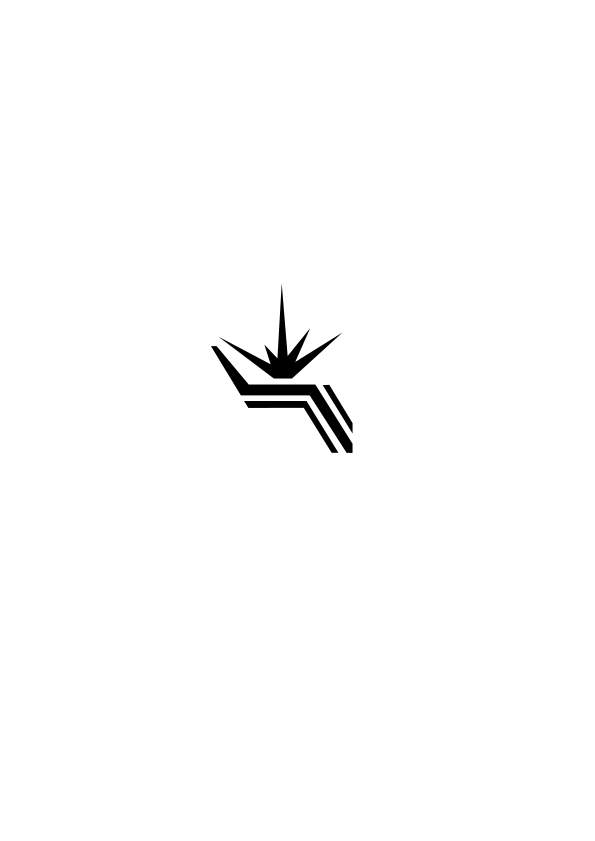
\includegraphics[width=\textwidth]{../BINP-logo}
    \end{minipage}\hfill
    \begin{minipage}{0.15\linewidth}
    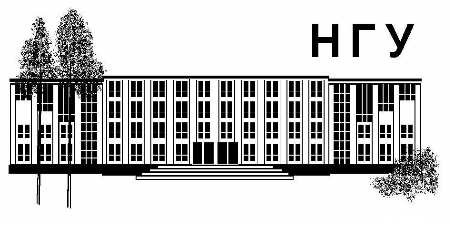
\includegraphics[width=\textwidth]{../NSU-logo}
    \end{minipage}
    \hfill
    \hspace*{5em}

    Кафедра теоретической физики физического факультета НГУ

    \large
    Профессор Фадин В.\,С.
    \vspace{-0.5em}

    \huge
    \textbf{Теория сильных взаимодействий}
    
    \Large
    Лекция № 12
    \vfill
    
    \normalsize
    \begin{minipage}{0.93\linewidth}
      \small Процессы электрон-позитронной аннигиляции в
      адроны. Экспериментальное открытие глюона в струйных
      событиях. Инклюзивные спектры. Инклюзивное сечение процесса с
      образованием фиксированного адрона $P$. Представление сечения в
      партонной модели. Функции фрагментации (число адронов
      в~партоне). Операторное разложение в следующем за главным
      логарифмическом приближении (СГЛП): неоднозначность, связанная
      с~зависимостью от масштаба перенормировки. Уравнение на функции
      фрагментации. Вычисление множественности (среднее количество
      адронов типа $P$): переход к моментам $M_j(Q^2)$, сингулярность
      при $x=0$, эффект когерентности излучения мягких глюонов,
      суммирование ряда теории возмущений в дважды логарифмическом
      приближении. Поведение моментов при $j\to 1$. Эффект «горбатого
      плато» в области малых $x$ в спектрах. Дисперсионные правила
      сумм. Вакуумные конденсаты. Нетривиальная структура вакуума
      КХД. Непертурбативные (невозмущенческие) эффекты. Дисперсионная
      связь $R$ и $P$ (поляризационного оператора). Необходимость
      введения глюонного конденсата.
    \end{minipage}
    \vfill
    
    \normalsize \ccbysa\hspace{0.5em} Новосибирск 2014   
  \end{center}
\end{titlepage}
\end{document}
